% vim: set textwidth=78 autoindent:

\subsection{Complemento fTools}\label{sec:ftools}

% when the revision of a section has been finalized, 
% comment out the following line:

La meta del complemento de python fTools es proveer recursos en un solo lugar para
muchas tareas com\'unes basadas en vectores, sin la necesidad de software adicional, 
librer\'{\i}as, o soluciones complejas. Provee una serie creciente de funciones 
de manejo espacial de datos y an\'alisis que son r\'apidas y funcionales. 

Ahora fTools se instala autom\'aticamente y activado en nuevas versiones de QGIS, y como con todos los complementos, puede 
ser desactivado y activado usando el Manejador de Complementos (Vea la secci\'on \ref{sec:managing_plugins}).
Cuando est\'a activado, el complemento fTools agrega un men\'u \mainmenuopt{Herramientas} a QGIS, proveyendo funciones que van desde 
Herramientes de An\'alisis e Investigaci\'on hasta herramientas de Geometr\'{\i}a y Geoprocesamiento, as\'{\i} como m\'ultiples utiles herramientas para el manejo de datos.

\minisec{Funciones de fTools}\label{ftool_functions}

Las tablas \ref{tab:ftool_analysis} a la \ref{tab:fTool_data_management} listan las funciones disponibles via el complemento fTools, junto con una breve descripci\'on de cada funci\'on. Para mas informaci\'on de una funci\'on individual de fTools, por favor haga clic en el elemento del men\'u \dropmenuopt{Informaci\'on de fTools} en el men\'u \mainmenuopt{Herramientas}.

\begin{table}[ht]\index{Analysis tools}
\centering
\caption{Herramientas de an\'alisis de fTools}\label{tab:ftool_analysis}\medskip
 \begin{tabular}{|p{0.3in}|p{1.2in}|p{4.7in}|}
 \hline \multicolumn{3}{|c|}{\textbf{Herramientas de an\'alisis via complemento fTools}} \\
 \hline \textbf{\'Icono} & \textbf{Herramienta} & \textbf{Prop\'osito} \\
 \hline 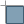
\includegraphics[width=0.7cm]{matrix} & Matriz de distancia &
Mide distancias entre dos capas de puntos, y da salida a los resultados como una a) matriz
de distancias cuadrada, b) Matriz de distancia lineal, or c) Resument de distancias. Puede limitar distancias
a los k objetos espaciales mas cercanos. \\ 
 \hline 
\includegraphics[width=0.7cm]{sum_lines} & Sumar longitud de l\'{\i}neas & Calcular
la suma total de las longitudes de l\'{\i}neas para cada pol\'{\i}gono de una capa vectorial de pol\'{\i}gonos. \\
 \hline 
\includegraphics[width=0.7cm]{sum_points} & Puntos en pol\'{\i}gonos & Cuenta el n\'umero
de puntos que ocurren en cada pol\'{\i}gono de una capa vectorial de pol\'{\i}gonos de entrada. \\
 \hline 
\includegraphics[width=0.7cm]{unique} & Listar valores \'unicos & Lista
todos los valores \'unicos de un campo en una capa vectorial de entrada. \\
 \hline 
\includegraphics[width=0.7cm]{basic_statistics} & Estad\'{\i}sticas b\'asicas & Calcula
estad\'{\i}sticas b\'asicas (mean, std dev, N, sum, CV) en un campo de entrada. \\ 
 \hline 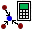
\includegraphics[width=0.7cm]{neighbour} & An\'alisis de vecinos mas proximos
& Calcula estad\'{\i}sticas de vecinos mas pr\'oximos para evaluar el nivel de agrupaci\'on en una
capa vectorial de puntos. \\
 \hline 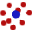
\includegraphics[width=0.7cm]{mean} & Coordenada(s) media &
Calcula bien la media normal o la media ponderada central de una capa vectorial completa,
o m\'ultiples objetos espaciales basados en un campo ID \'unico. \\ 
 \hline 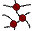
\includegraphics[width=0.7cm]{intersections} & Intersecciones de l\'{\i}nea &
Localiza intersecciones entre l\'{\i}neas, y da salida a resultados como un shapefile de puntos.
\'Util para localizar calles o intersecciones de corrientes, ignora intersecciones de l\'{\i}nea
con longitud > 0. \\
 \hline
\end{tabular}
\end{table}

\begin{table}[ht]\index{Research tools}
\centering
\caption{Herramientas de investigaci\'on de fTools}\label{tab:ftool_research}\medskip
 \begin{tabular}{|p{0.3in}|p{1.3in}|p{4.6in}|}
 \hline \multicolumn{3}{|c|}{\textbf{Herramientas de investigaci\'on disponibles via el complemento fTools}} \\
 \hline \textbf{Icon} & \textbf{Herramienta} & \textbf{Prop\'osito} \\
 \hline 
\includegraphics[width=0.7cm]{random_selection} & Selecci\'on aleatoria & Aleatoriamente 
selecciona n n\'umeros de objetos espaciales, o n porcentajes de objetos espaciales \\
 \hline 
\includegraphics[width=0.7cm]{sub_selection} & Selecci\'on aleatoria dentro de
 subconjuntos & Aleatoriamente selecciona objetos espaciales dentro de subconjuntos basados en campo ID \'unico. \\
 \hline 
\includegraphics[width=0.7cm]{random_points} & Puntos aleatorios & Genera 
puntos seudo-aleatorios sobre una capa de entrada dada. \\
 \hline 
\includegraphics[width=0.7cm]{regular_points} & Puntos regulares & Genera 
una rejilla regular de puntos sobre una regi\'on especificada y los exporta como un shapefile de puntos. \\
 \hline 
\includegraphics[width=0.7cm]{vector_grid} & Cuadr\'{\i}cula vectorial & Genera una 
l\'{\i}nea o cuadr\'{\i}cula de pol\'{\i}gono basado en un espaciado de cuadr\'{\i}cula especificado por el usuario. \\
 \hline 
\includegraphics[width=0.7cm]{select_location} & Seleccionar por localizaci\'on & 
Selecciona objetos espaciales basados en su localizaci\'on relativa a otra capa para formar una 
nueva selecci\'on, o agregar o substraer desde la selecci\'on actual. \\
\hline 
\includegraphics[width=0.7cm]{layer_extent} & Pol\'{\i}gono desde extensi\'on de capa & 
Crea un pol\'{\i}gono rectangular desde la extensi\'on de una capa raster o vectorial de entrada. \\
 \hline
\end{tabular}
\end{table}

\begin{table}[ht]\index{Geoprocessing tools}
\centering
\caption{Herramientas de geoproceso de fTools}\label{tab:ftool_geoprocessing}\medskip
 \begin{tabular}{|p{0.3in}|p{0.8in}|p{5.1in}|}
 \hline \multicolumn{3}{|c|}{\textbf{Herramientas de geoproceso disponibles via el complemento fTools}} \\
 \hline \textbf{Icon} & \textbf{Herramienta} & \textbf{Prop\'osito} \\
 \hline 
\includegraphics[width=0.7cm]{convex_hull} & Convex hull(s) & Crea 
convex hull(s) m\'{\i}nimos para una capa de entrada, o basado en un campo ID. \\
 \hline 
\includegraphics[width=0.7cm]{buffer} & Buffer(s) & Crea 
buffer(s) alrededor de objetos espaciales basado en distancia, o campo distancia. \\
 \hline 
\includegraphics[width=0.7cm]{intersect} & Intersecci\'on & Sobrepone 
capas de manera que la salida contiene \'areas donde ambas capas se intersectan. \\
 \hline 
\includegraphics[width=0.7cm]{union} & Uni\'on & Sobrepone capas de manera que 
dan como salida \'areas de intersecc\'on y no intersecci\'on. \\
 \hline 
\includegraphics[width=0.7cm]{sym_difference} & Diferencia sim\'etrica & 
Sobrepone capas de manera que la salida contiene esas \'areas de la capa de entrada y capa 
de diferencia que no se intersectan.\\
 \hline 
\includegraphics[width=0.7cm]{clip} & Cortar & Sobrepone capas de manera 
que la salida contiene \'areas que intersectan la capa a cortar. \\
 \hline 
\includegraphics[width=0.7cm]{difference} & Diferencia & Sobrepone capas 
de manera que la salida contiene \'areas que no se intersectan con la capa de corte. \\
 \hline 
\includegraphics[width=0.7cm]{dissolve} & Disolver & Une objetos espaciales 
basados en un campo de entrada. Todos los objetos espaciales con valores de entrada identicos son combinados 
para formar un solo objeto espacial. \\
 \hline
\end{tabular}
\end{table}

\begin{table}[ht]\index{Geometry tools}
\centering
\caption{Herramientas de geometr\'{\i}a de fTools}\label{tab:ftool_geometry}\medskip
 \begin{tabular}{|p{0.3in}|p{1.2in}|p{4.8in}|}
 \hline \multicolumn{3}{|c|}{\textbf{Herramientas de geometr\'ia disponibles via el complemento fTools}} \\
 \hline \textbf{Icon} & \textbf{Tool} & \textbf{Purpose} \\
 \hline 
\includegraphics[width=0.7cm]{check_geometry} & Comprobar validez de geometr\'{\i}a & 
Comprueba pol\'{\i}gonos para intersecciones, huecos cerrados, y orden fijo de nodos. \\
 \hline 
\includegraphics[width=0.7cm]{export_geometry} & Exportar/A\~nadir columnas de geometr\'{\i}a 
& A\~nade informaci\'on de geometr\'{\i}a de capa vectorial a capas de punto (XCOORD, YCOORD), 
de l\'{\i}nea (LONGITUD), o pol\'{\i}gono (\'AREA, PER\'IMETRO). \\
 \hline 
\includegraphics[width=0.7cm]{centroids} & Centroides de pol\'{\i}gonos & 
Calcula los centroides verdaderos para cada pol\'{\i}gono en una capa de entrada de  for each polygon in an input polygon layer. \\
 \hline 
\includegraphics[width=0.7cm]{delaunay} & Triangulaci\'on Delaunay & 
Calcula y da salica (como pol\'{\i}gonos) la triangulaci\'on delaunay de una capa vectorial de entrada. \\
 \hline 
\includegraphics[width=0.7cm]{simplify} & Simplificar geometr\'{\i}a & 
Generaliza l\'{\i}neas o pol\'{\i}gonos con un algoritmo modificado Douglas-Peucker. \\
 \hline 
\includegraphics[width=0.7cm]{multi_to_single} & Multiparte a 
partes sencillas & Convierte objetos espaciales multiparte a m\'ultiples objetos espaciales simples. 
Crea pol\'{\i}gonos y l\'i{\i}neas simples. \\
 \hline 
\includegraphics[width=0.7cm]{single_to_multi} & Partes sencillas a 
multiparte & Une m\'ultiples objetos espaciales a objeto espacial multiparte basado 
en un campo ID \'unico. \\
 \hline 
\includegraphics[width=0.7cm]{to_lines} & Pol\'{\i}gonos a l\'{\i}neas 
& Convierte pol\'{\i}gonos a l\'{\i}neas, pol\'{\i}gonos multiparte a  m\'ultiples l\'{\i}neas simples. \\
 \hline 
\includegraphics[width=0.7cm]{extract_nodes} & Extraer nodos & 
Extrae nodos desde capas de l\'{\i}neas y pol\'{\i}gonos y les da salida como puntos. \\
 \hline
\end{tabular}
\end{table}

\begin{table}[ht]\index{Data management tools}
\centering
\caption{Herramientas de manejo de datos de fTools}\label{tab:fTool_data_management}\medskip
 \begin{tabular}{|p{0.3in}|p{1.3in}|p{4.6in}|}
 \hline \multicolumn{3}{|c|}{\textbf{Herramientas de manejo de datos disponibles via el complemento fTools}} \\
 \hline \textbf{Icon} & \textbf{Herramienta} & \textbf{Prop\'osito} \\
 \hline 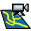
\includegraphics[width=0.7cm]{export_projection} & Exportar a nueva proyecci\'on & 
Proyecta objetos espaciales a un nuevo SRC y los exporta como un nuevo shapefile. \\
 \hline 
\includegraphics[width=0.7cm]{define_projection} & Definir la proyecci\'on actual & 
Specifica leSRC para shapefiles cuyo SRC no ha sido definido. \\
 \hline 
\includegraphics[width=0.7cm]{join_attributes} & Unir atributos & Une 
atributos adicionales a la tabla de atributos de capas vectoriales y da salida a los resultados
a un nuevo shapefile. Aditionalmente los atributos pueden ser desde una capa vectorial o 
desde una tabla dbf. \\
 \hline 
\includegraphics[width=0.7cm]{join_location} & Unir atributos por
localizaci\'on & Une atributos adicionales a una capa vectorial basada en 
relaciones espaciales. Atributos desde una capa vectorial son agregados a la tabla de atributos 
de otra capa y exportados como un shapefile \\
 \hline 
\includegraphics[width=0.7cm]{split_layer} & Dividir capa vectorial & 
Divide un capa de entrada en m\'ultiples capas separadas basado en un campo de entrada. \\
 \hline
\end{tabular}
\end{table}



